% ==================================================
% CHAPTER 3: The LHC and the ATLAS experiment %
% ==================================================

\chapter{The LHC and the ATLAS experiment}
\label{chap:lhc_atlas}

The Large Hadron Collider (LHC) is the world's most energetic particle accelerator and the ATLAS experiment is used to record the results of particle collisions at the LHC. In this chapter, details about both that are necessary to understand the High-Luminosity LHC (HL-LHC) upgrade project and the ATLAS experiment's New Small Wheels (NSWs) upgrade are presented.

% --------------------------------------------------
\section{The Large Hadron Collider}
% --------------------------------------------------

The LHC is an accelerator \SI{27}{\kilo\meter} in circumference and located $\sim$\SI{100}{\meter} underground at the CERN laboratory near Geneva, Switzerland~\cite{evans_lhc_2008}. It has two beam pipes within which bunches of protons counter-circulate before being collided in the center of one of four major experiments, such as the ATLAS experiment (discussed in section~\ref{sec:atlas}). Protons are guided on the circular trajectory using 1232 superconducting dipole magnets capable of a maximum field of \SI{8.33}{T}. Radio-frequency accelerating cavities are used to accelerate protons to a the maximum design energy of 7 TeV~\cite{bruning_lhc_2004}.  During LHC Run-1 (2011-2012), protons were collided at a collision center-of-mass energy of 7 TeV and 8 TeV~\cite{atlas_luminosity_run1}. During LHC Run-2 (2015-2018), the center-of-mass energy of proton collisions was increased to 13 TeV~\cite{atlas_luminosity_run2}, close to the maximum design value of 14 TeV~\cite{bruning_lhc_2004}. It is not actually the protons that interact, but the constituent quarks and gluons that each carry some fraction of the energy and momentum of the collisions.

% There are two main branches of study that can be pursued with the LHC and ATLAS. First, properties predicted by the standard model (SM) of particle physics can be measured. Else, physicists can search for evidence of processes predicted by theories beyond the standard model. Both the SM measurement and search analyses are based on measuring the number of times a given process occurs and comparing it to expectations. In this way, the number of proton-proton interactions created by the LHC directly affects the statistics available to do SM measurements and searches using the ATLAS experiment.

\paragraph*{Luminosity} \hfill \break
The number of proton-proton interactions generated by the LHC directly affects the statistics available to make measurements of interaction cross sections.
%IF YOU DON'T NEED TO DEFINE LUMINOSITY
% The number of interactions is quantified by luminosity, a property of the accelerator and its operating conditions~\cite{zyla_review_2020}. When the instantaneous luminosity is integrated over a data collection period and multiplied by the cross section of a given process, the result is the expected number of times that process occurs (so luminosity has units of inverse cross section). Since luminosity is derived from the accelerator parameters, it is the link between the machine and the statistical power of potential measurements. 
% IF YOU NEED TO DEFINE LUMINOSITY
% THIS SECTION IS NOT CITED, probably cite wiht zyla_review_2020
Predicting the number of proton-proton interactions requires defining a metric called luminosity~\cite{zyla_review_2020}. The luminosity of a particle collider is the number of particles an accelerator can send through a given area per unit time. It is calculated from the measurable quantities in Equation~\ref{eqn:inst_lum}:

\begin{equation}
\mathcal{L} = \frac{f N_{1} N_{2} }{4 \pi \sigma_{x} \sigma_{y}}~,
\label{eqn:inst_lum}
\end{equation}

where $f$ is the frequency of the bunch crossings (\SI{25}{\nano\second}), $N_{1}$ and $N_{2}$ are the number of protons in each bunch ($\sim 10^{11}$ protons / bunch), and $\sigma_{x}$ and $\sigma_{y}$ are the RMS of the spatial distributions of the bunch. Therefore, luminosity is a property of accelerator beams, which are set by the capabilities of the accelerator. The design luminosity of the LHC was $10^{34}$~cm$^{-2}$s$^{-1}$. The units of luminosity are an inverse area; multiplying the luminosity by the cross section of a given process gives the expected rate for that process.

Integrating the \textit{instantaneous} luminosity (equation~\ref{eqn:inst_lum}) over a period of data collection time gives the integrated luminosity,

\begin{equation}
L = \int \mathcal{L} \left( t \right) \,dt
\label{eqn:int_lum}
\end{equation}

which is related to the total number of interactions. In this way, the luminosity is the link between the accelerator and the statistical power of measurements to be made with the data collected. So far, the LHC provided an integrated luminosity of \SI{28.26}{\per\femto\barn} in Run-1~\cite{atlas_luminosity_run1} and \SI{156}{\per\femto\barn} in Run-2~\cite{atlas_luminosity_run2}.

% --------------------------------------------------
\section{The High-Luminosity LHC}
% --------------------------------------------------
At the end of the LHC program in 2025, the statistical gain on measurements in running the LHC further will become marginal. The HL-LHC~\cite{hl_lhc_tdr} project consists of the upgrade of LHC infrastructure to achieve a nearly ten fold increase in instantaneous luminosity, thereby improving measurement statistics as well. Also, some systems will need repair and replacement to operate past $\sim$2020. The LHC will continue to be the most energetic accelerator in the world for years to come and is the only accelerator with enough energy to directly produce the Higgs boson and top quarks. Therefore, the European Strategy for Particle Physics made it a priority ``to fully exploit the physics potential of the LHC'' with ``a major luminosity upgrade''~\cite{european_strategy_for_particle_physics}. The goal is for the HL-LHC to provide an integrated luminosity of \SI{3000}{\per\femto\barn} in the 12 years following the upgrade. The luminosity actually achieved will depend on a combination of technological advances and upgrades in progress that affect the factors contributing to luminosity defined in equation~\ref{eqn:inst_lum}~\cite{hl_lhc_tdr}. Figure~\ref{fig:hl-lhc} shows the projected schedule of the HL-LHC upgrades and operation~\cite{hl-lhc_plan_picture_website}.

\begin{figure}
    \centering
    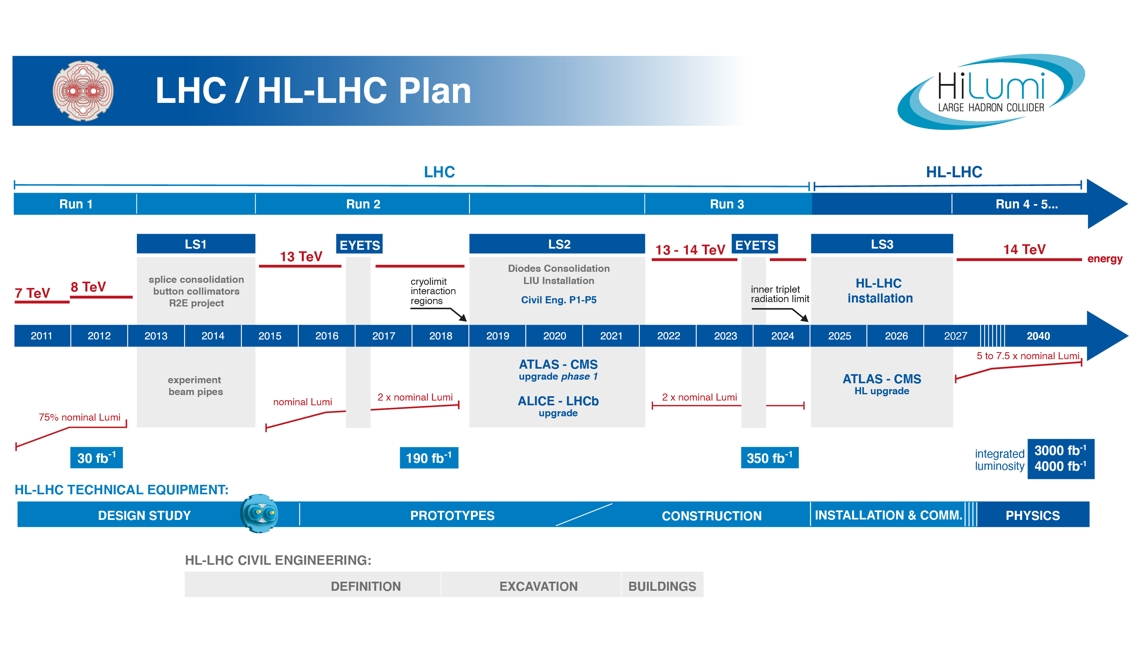
\includegraphics[width = \textwidth]{figures/HL-LHC-updated-January-2021_small.jpg}
    \caption{The LHC/HL-LHC timeline~\cite{hl-lhc_plan_picture_website}. The integrated luminosities collected and projected for each run of the LHC are shown in blue boxes below the timeline and the center of mass energy of the collisions is shown in red above the timeline. The top blue arrow labels the run number. The acronym ``LS'' stands for ``long shutdown'' and indicates periods where the accelerator is not operating. During the shutdowns, upgrades to the LHC and the experiments are taking place. This timeline was last updated in January, 2021, and reflects changes in the schedule due to the ongoing pandemic. }
    \label{fig:hl-lhc}
\end{figure}

% The increase in statistics the HL-LHC will improve measurements of standard model parameters and improve searches for unobserved phenomena~\cite{dainese_physics_2018}. A particular measurement that will benefit from the increased statistics is of the triple-Higgs coupling. Measuring the coupling measures the shape of the Higgs potential responsible for electroweak symmetry breaking. Any discrepancy with the SM prediction will show that there must be other sources of electroweak symmetry breaking~-- if there is such another source, it could be an avenue to study the other questions the SM does not address. Also, the sensitivity to several exotic Higgs decays to BSM particles will be improved. Many of the products of exotic Higgs decays are dark matter candidates or otherwise could extend the scope of the SM.

% Higgs couplings to particles will all be measured to the percent level at the HL-LHC and sensitivity to SM predicted Higgs decays will increase. Also, the sensitivity to several exotic Higgs decays to BSM particles will be improved. Many of the products of exotic Higgs decays are dark matter candidates or otherwise could extend the scope of the SM. The LHC is the only accelerator energetic enough to directly produce Higgs bosons, so it is the only tool able to probe questions about the Higgs.

One of the most anticipated measurements at the HL-LHC is the value of the triple-Higgs coupling. Measuring the coupling will allow the determination of the shape of the Higgs potential responsible for electroweak symmetry breaking. Any discrepancy with respect to the SM prediction will show that there must be other sources of electroweak symmetry breaking, and hence physics phenomena beyond the SM. The LHC is the only accelerator where the Higgs boson can be produced directly so it is the only place where the triple-Higgs coupling could be measured. The HL-LHC upgrade is required to produce a significant sample of Higgs produced in pairs to make a statistically meaningful measurement~\cite{dainese_physics_2018, cepeda_report_2018}. Accordingly, detector sensitivity to various Higgs decays will be important at the HL-LHC.
%The estimated number of interactions of a given type per bunch crossing is given by equation~\ref{eqn:num_interactions}.
%\begin{equation}
%\mu = \sigma \delta t\mathcal{L}
%\label{eqn:num_interactions}
%\end{equation}

% The energies accessible by the accelerator make it unique infrastructure with which to study processes of the standard model of particle physics and search for new phenomenon beyond the standard
% model. Considerable progress has been made towards answering the questions originally used to motivate the construction of the LHC, but many remain unanswered or only partially answered~ \cite{brianti_large_1984}. Therefore, the continued use and maintenance of the accelerator 

% --------------------------------------------------
\section{The ATLAS experiment}
% --------------------------------------------------
\label{sec:atlas}

The ATLAS experiment~\cite{collaboration_atlas_2008} was designed to support all the physics goals of the LHC. It is \SI{44}{\meter} long and \SI{25}{\meter} in diameter, and weighs 7000 tonnes. The ATLAS experiment is centered around one of the LHC's interaction points (a place where the beams collide). As shown schematically in figure~\ref{fig:atlas}, ATLAS consists of an array of particle detector subsystems arranged concentrically around the beam pipe.  The ATLAS experiment is cylindrical because it aims to provide 4$\pi$ coverage around the interaction point. In reference to the cylindrical geometry of the experiment, it is helpful to separate the subsystems of ATLAS into the so-called ``barrel'' and ``endcap''/``forward'' regions.

\begin{figure}
    \centering
    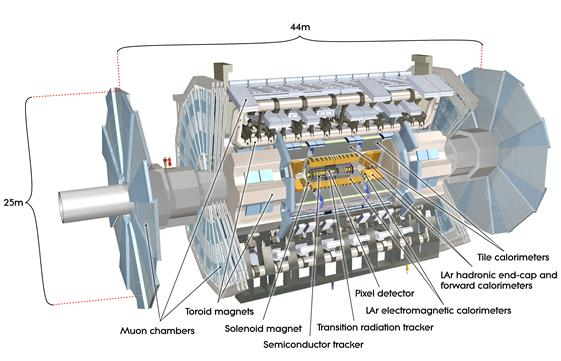
\includegraphics[width = \textwidth]{figures/atlas_diagram.png}
    \caption{Schematic diagram of the ATLAS experiment, with the various detector subsystems labelled~\cite{collaboration_atlas_2008}.}
    \label{fig:atlas}
\end{figure}

For analysis purposes, a spherical coordinate system is defined. The azimuthal angle $\phi$ is measured around the beampipe and the polar angle $\theta$ is measured from the beam pipe. The polar angle is more often expressed in terms of pseudo-rapidity, defined as $\eta = -\ln\tan\left(\theta/2\right)$.  Pseudo-rapidity values vary from 0 (perpendicular to the beam) to $\pm\infty$ (parallel to the beam, defined as the z-direction) and is an approximation to the rapidity of a particle when its momentum is much greater than its mass. It is useful to describe the direction of outgoing particles in proton-proton collisions because differences in rapidity are invariant to a Lorentz boost along the beam direction.

The ATLAS experiment provides identification and kinematic measurements for each particle created after the initial collision, which is done by assembling offline the information recorded by each subsystem. With this information, signatures of processes of interest can be identified and studied. An overview of the main ATLAS subsystems is given below.

\paragraph*{The inner detector} \hfill \break
The inner detector~\cite{atlas_inner_detector_tdr_1, atlas_inner_detector_tdr_2} (figure~\ref{fig:atlas_inner_detector}) is for precise measurements of charged particle trajectories, measurement of primary and secondary interaction vertices and assistance in the identification of electrons. A \SI{2}{\tesla} solenoid with field parallel to the beam bends the trajectory of outgoing charged particles. A measurement of the bending radius of each charged particle provides information about its momentum. The innermost part of the inner tracker is made of high-resolution semiconductor pixel and strip detectors while the outermost part is made of straw-tubes. The straw tubes are used in the trajectory measurements but they are also interspersed with material designed to enhance the creation of transition radiation. Transition radiation occurs when a highly relativistic charged particle traverses a material boundary~\cite{grupen_particle_2008}. The amount of transition radiation emitted by a charged particle is detected by the straw-tubes and is used to identify electrons. 

\begin{figure}
    \centering
    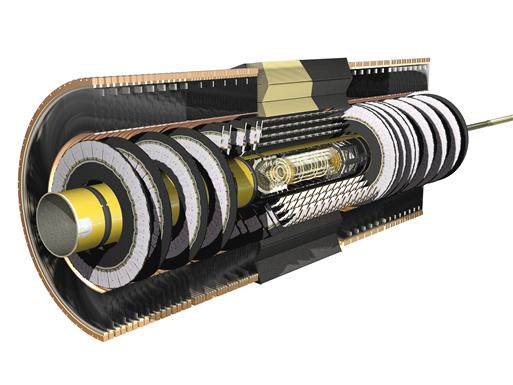
\includegraphics[width = 0.5\textwidth]{figures/atlas_inner_detector.jpg}
    \caption{Schematic diagram of the ATLAS experiment's inner detector, with the different segments and the technology used labeled~\cite{collaboration_atlas_2008}.}
    \label{fig:atlas_inner_detector}
\end{figure}

% YOU ARE HERE
\paragraph*{Calorimetry system} \hfill \break
Electromagnetic and hadronic sampling calorimeter units are used to record the energy of electrons, photons and jets\footnote{When quarks or gluons are expelled in a high energy collsion, they create collimated groups of hadrons because they carry a charge called ``colour'', and nature only allows ``colourless'' combinations to exist~\cite{grupen_particle_2008}.}. A combination of liquid-argon (LAr) electromagnetic and hadronic calorimeters~\cite{atlas_lar_cal_tdr} and tile-scintillator hadronic calorimeters~\cite{atlas_tile_cal_tdr} cover the rapidity range $|\eta| < 4.9$, as shown in figure~\ref{fig:atlas_calorimeter}.

\begin{figure}
    \centering
    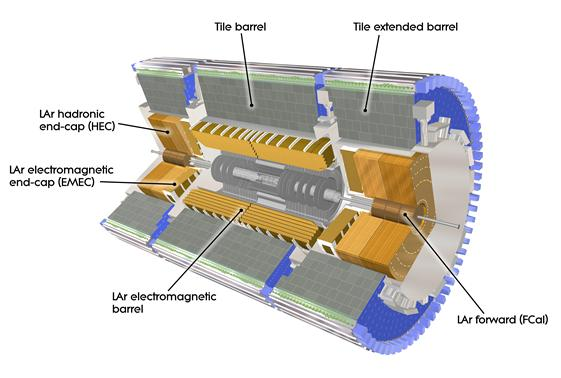
\includegraphics[width = 0.5\textwidth]{figures/atlas_calorimeter.png}
    \caption{Schematic diagram of the ATLAS calorimeter system, with the different segments and the technology used labeled~\cite{collaboration_atlas_2008}.}
    \label{fig:atlas_calorimeter}
\end{figure}

Sampling calorimeters have alternating layers of dense material and material that can measure the amount of ionization by charged particles. The dense material causes incoming charged particles to shower into lower energy particles and deposit their energy in the sensitive volume. Only muons and neutrinos are known to pass the calorimeters to the muon spectrometer without being absorbed. 

\paragraph*{Muon spectrometer} \hfill \break
The muon spectrometer~\cite{atlas_muon_spectrometer_tdr} consists of multiple layers of tracking chambers embedded in a 2 T magnetic field generated by an air-core superconducting toroid magnet system. Figure~\ref{fig:atlas_muon_spectrometer_3D} shows a schematic diagram of the layout of the different chambers and of the toroid magnets~\cite{collaboration_atlas_2008}. The trajectory of a muon is reconstructed from the information recorded by the different types and layers of tracking chambers. The amount of bending in the magnetic field provides a measure of the muon's momentum. In the barrel section of ATLAS, the toroidal magnetic field is created by eight coils bent into the shape of a  "race-track"  and symmetrically arranged around the beampipe.  In the forward region, two end-cap toriods, each with eight smaller racetrack-shaped coils arranged symmetrically around the beam pipe are inserted in the ends of the barrel toroid~\cite{atlas_magnet_tdr}.

\begin{figure}
\centering
\begin{subfigure}{.5\textwidth}
  \centering
  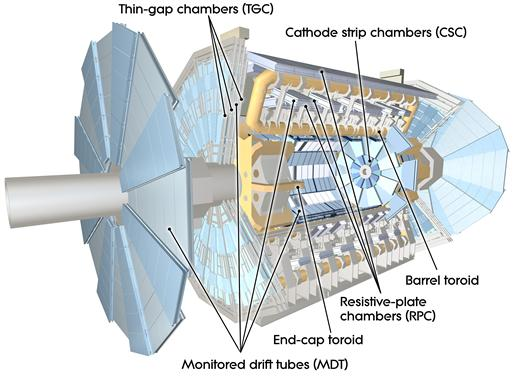
\includegraphics[width=\linewidth]{figures/atlas_muon_spectrometer.jpg}
  \caption{}
  \label{fig:atlas_muon_spectrometer_3D}
\end{subfigure}%
\begin{subfigure}{.5\textwidth}
  \centering
  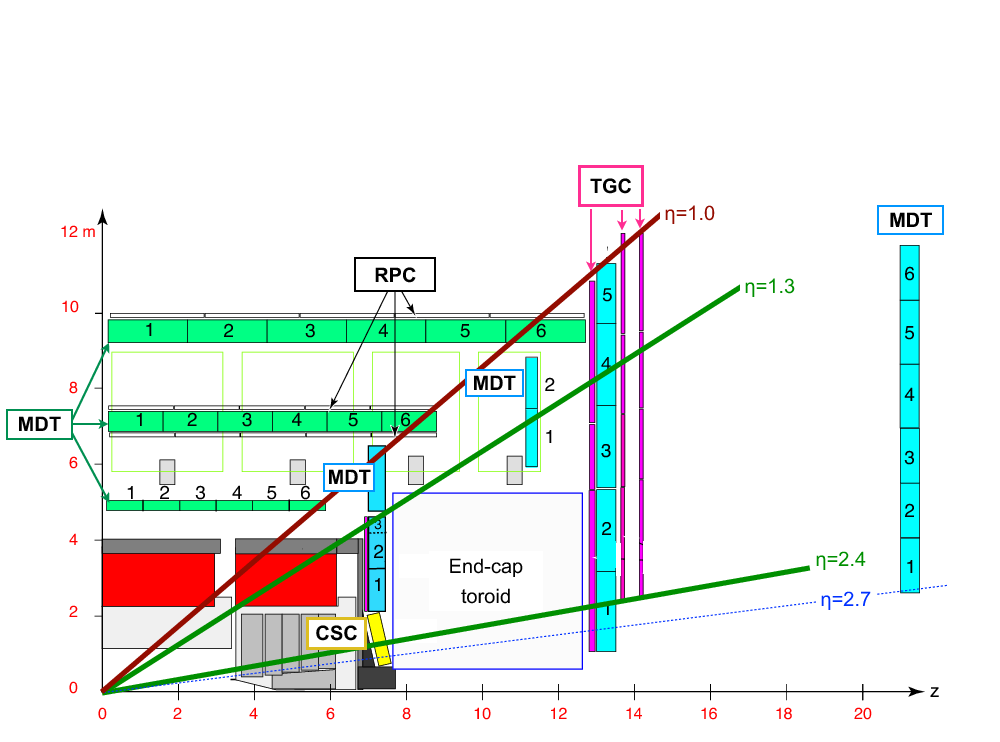
\includegraphics[width=\linewidth]{figures/atlas_old_muon_spec_quarter_cut_recolour.png}
  \caption{}
  \label{fig:atlas_muon_spectrometer_cut}
\end{subfigure}
\caption{Schematic diagram of the ATLAS muon spectrometer. Figure~(a) shows a 3D projection of the system with the different types of chambers and different parts of the toroidal magnet system labeled~\cite{collaboration_atlas_2008}. Figure~(b) shows a projection of one quarter of the muon spectrometer, with the interaction point in the bottom left corner. The small wheel is just left of the end cap toroid, the big wheel is to its right, and the outer wheel is the rightmost structure~\cite{atlas_performance_muon_trigger_2015}.}
\label{fig:atlas_muon_spectrometer}
\end{figure}

The muon spectrometer is separated into detectors used for precision offline tracking and for triggering purposes. Three layers of monitored drift tubes (MDTs) or cathode strip chambers (CSCs) are used for tracking. The position of the muon track in each of the three layers allows reconstruction of the bent trajectory of a muon and hence its momentum. To satisfy the muon spectrometer target momentum resolution of $\Delta p_T / p_T <$~1$\times$10$^{-4}~p$~/~GeV for $p_T <$~300~GeV and a few percent for lower $p_T$ muons, the MDTs and CSCs were designed to achieve a spatial resolution of \SI{50}{\micro\meter} each. Accordingly, an optical alignment system was designed to monitor and correct for chamber positions~\cite{atlas_muon_spectrometer_tdr, aefsky_optical_2008}. 

% Precision tracking is done offline for events passing the muon trigger. Each of the barrel and encap systems have three layers of MDTs that record the position of the muon as it passes through each layer. Knowing the magentic field, the muon's momentum can be extracted. For the design momentum resolution of $\Delta p_T / p_T <$ 1$\times$10$^{-4}~p$ / GeV for $p_T < 300 GeV$ and a few percent for lower $p_T$ muons, the MDTs and CSCs required position resolution of \SI{50}{\micro\meter} each. Accordingly, an optical alignment system was designed to monitor and correct for chamber positions~\cite{atlas_muon_spectrometer_tdr, aefsky_optical_2008}. 

% ON MUON TRIGGERING IN THE ENDCAP
% Decide how you want to do this based on the next section.
% At least 2 TGC layers in coincidence comes from muon spectrometer TDR; coincidence with "forward inner" detectors (small wheel) comes from Run-2 trigger upgrades paper, Martinez.
% NSW TDR says there are TGC layers in the small wheel that are the forward inner detectors added to Run-2 triggering.
% \textcolor{red}{The Run-2 L1 muon trigger was passed if TGC layers (two for low $p_T$ muons, three for high $p_T$ muons) of the big wheel fired in coincidence with a hit from the MDTs of the small wheel on the order of the bunch crossing time. The regions of interest defined by the TGCs were fed into the HLT, where MDT and TGC data could be combined for further cuts. The $p_T$ resolution of the L1 trigger is improved by the MDT tracking information. \textit{I'll decide how I want to do this after writing the motivation for the NSW}}
Resistive plate chambers (RPCs) are used for triggering in the barrel and thin-gap chambers (TGCs) are used for triggering in the endcaps. The positions of each type of chamber are sketched in figure~\ref{fig:atlas_muon_spectrometer_cut}. The endcap section of the muon spectrometer consists of three sections, the small wheel, big wheel, and outer wheel~-- ordered by proximity to the interaction point. In Run-1, low (high) $p_T$ muons were triggered on if two (three) of the RPC or TGC layers around the big wheel fired in coincidence, for the barrel and endcaps respectively~\cite{atlas_l1_trigger_tdr}. After Run-1 it was discovered that up to 90\% of the triggers in the endcap were fake, caused by background particles generated in the material between the small wheel and the big wheel~\cite{nsw_tdr}.  To reduce the fake rate in Run-2, the TGCs on the inside of the small wheel also had to register a hit. The added condition reduced the trigger rate by 50\% in the range 1.3 $< |\eta| <$ 1.9~\cite{martinez_run-2_2016}. The effectiveness of the solution was limited since the $|\eta|$-range of the small wheel TGCs was limited to 1.0 $< |\eta| <$ 1.9 and the spatial resolution of the small wheel TGCs is coarse~\cite{nsw_tdr}.

% In the barrel, three layers of MDTs are used for precision tracking, and resistive plate chambers (RPCs) are used for triggering. The endcaps of the muon spectrometer are composed of three wheels each, the small wheel (SW), big wheel, and outer wheel. All three wheels use MDTs for precision offline tracking, but cathode strip chambers (CSCs) are used in the forward region of the small wheel because they can better handle the increased background. Thin gap  chambers

% The big wheel and the outer wheel have MDTs for offline precision tracking and the thin gap chambers (TGCs) on either side for triggering. In the first two runs of ATLAS, offline precision tracking on the small wheel was done with MDTs and cathode strip chambers (CSCs), and their output did not contribute to the trigger.~\cite{atlas_muon_spectrometer_tdr}. 

% Sentences if you go without 1/4 cut figure
% In the barrel, three layers of monitored drift tubes (MDTs) are arranged between, above and below the barrel toroid magnets. They are used for precision tracking. On both sides of the middle layer of  MDTs and on the top of the top layer of MDTs are resitive plate chambers (RPCs), used for triggering.
%  The inner part had cathode strip chambers (CSCs), which had higher granularity to handle the increased background radiation rate in the forward region

% The muon spectrometer is the outermost layer of the ATLAS detector, since only muons (and neutrinos) can pass through the calorimeters. For muons that are ejected towards the end-caps of ATLAS, their trajectory is bent by the magentic field and their position recorded by three successive wheels of muon detectors. With each wheel providing the position of the muon along its trajectory and knowledge of the magentic field, the momentum of the muon generated in the collision can be reconstructed. 

\paragraph*{Trigger system} \hfill \break
It would be impossible to record all the data from bunch crossings every \SI{25}{\nano\second}, corresponding to a rate of $\sim$\SI{40}{MHz}. The ATLAS experiment has a multi-level trigger system to select events of interest for permanent storage. The Level-1 (L1) hardware trigger~\cite{atlas_l1_trigger_tdr} uses partial-granularity information from the muon spectrometer and calorimeters to trigger on high $p_T$ muons, electrons, jets, missing transverse energy, and $\tau$ decaying to hadrons. After Run-3 an upgrade of the trigger system will allow a maximum trigger rate of \SI{1}{MHz} with a latency of \SI{10}{\micro\second}~\cite{tdaq_phase2_tdr}, but for now the working limits are a rate of \SI{100}{kHz}~\cite{martinez_run-2_2016} and \SI{2.5}{\micro\second}~\cite{atlas_l1_trigger_tdr}.

% The Level-1 (L1) hardware trigger uses the muon spectrometer's TGCs and RPCs to trigger on high $p_T$ muons and the calorimeter detector units to trigger on electrons, jets, high missing transverse energy, and $\tau$ decaying to hadrons, with a maximum trigger rate of \SI{100}{kHz} and latency of \SI{2.5}{\micro\second}. The L1 trigger only uses a fraction of the granularity offered by the detectors.

The L1 trigger is used to define regions of interest that are fed into the software high level trigger (HLT)~\cite{atlas_hlt_trigger_tdr}, in which the full granularity of the muon spectrometer and calorimeter are used with information from the inner detector to reduce the trigger rate to 1 kHz. Events that satisfy at least one of the L1 and HLT trigger criteria are recorded to permanent storage for offline analysis.

% Paragraph separator line
\begin{center}
  \noindent\rule[0.5ex]{0.1\linewidth}{0.5pt}
\end{center}

With the foreseen increase in luminosity at HL-LHC, it is a priority to upgrade the ATLAS detector to further reduce the muon trigger fake rate in the forward region. The New Small Wheels being commissioned to replace the original ATLAS muon small wheels will address this challenge.